\section{\dReach{}: System Description}
\begin{figure}
  \centering
  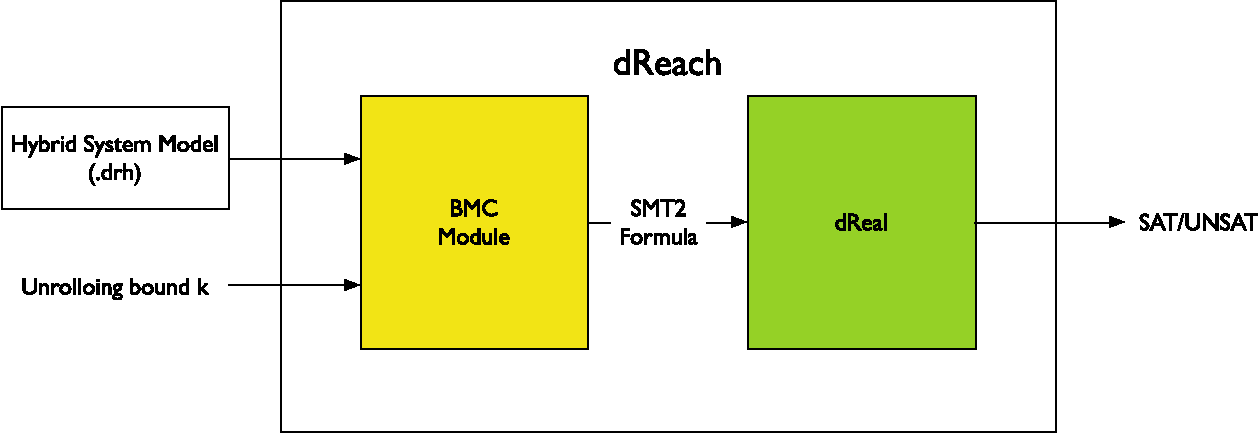
\includegraphics[width=\textwidth]{images/dReach}
  \caption{Architecture of \dReach{}: It consists of an bounded
    model-checking module and an SMT solver, \dReal{}. In the first
    phase, the BMC module translate an input hybrid system into a
    logic formula with respect to the specified unrolling bound $k$
    and the provided reachability condition $\textit{goal}$ in the
    model. In the second phase, an SMT solver, \dReal{}, solves the
    encoded $\delta$-reachability problem.}
  \label{fig:system-description}
\end{figure}

Figure~\ref{fig:system-description} illustrates the architecture of
\dReach{}. We provide a domain-specific lanaguage to describe a hybrid
system and specify its safety properties. Given an input model,
specification, and unrolling bound $k$, \dReach{} reduces the
$\delta$-reachability problem to a $\delta$-decision problem of
formulae over the reals by providing a corresponding SMT encoding for
the problem. Then, the bounded reachability queries are answered by
using our nonlinear SMT solver \dReal{}~\cite{DBLP:conf/cade/GaoKC13}.

\subsection{Encoding Bounded Reachability Problem}

Our previous work~\cite{DBLP:journals/corr/GaoKCC14} already studied
logic encodings of bounded reachability problems of hybrid
systems. The encoding scheme is based on the standard bounded model
checking while non-trivial mode invariants and systems with
nondeterministic flows make the problem interesting.

In this section, we explain the extensions and variable naming
convention that we make to the standard SMT-LIB~\cite{BarST-SMT-10} to
represent flows and mode invariants of hybrid systems.

\paragraph{Variable naming convention}
In our encoding, a system variable $\texttt{x\_i\_p}$ has two
subscripts $i \in \mathbb{N}$ and $p \in \{0, t\}$. The first
subscript $i$ indicates that it represents the value of a system
variable $x$ at the $i$-th step. The second subscript $p \in \{0, t\}$
denotes the value at the begining of mode (end of mode,
respectively). For instance, $x\_0\_t$ denotes the value of variable
$x$ at the end of first mode (step 0).

\paragraph{define-ode and integral}
A flow consists of a group of ordinary differential equations. In
\drh{}, we provide a command \texttt{define-ode} to associate a flow
with a name. For instance, we use $\texttt{define-ode}$ as follows to
assign a name $\mathrm{flow_1}$ to a group of ODE,
$\frac{\mathrm{d}x}{\mathrm{d}t} = v$ and
$\frac{\mathrm{d}v}{\mathrm{d}t} = -9.8$.
\[
\texttt{(define-ode flow\_1 ((= d/dt[x] v) (= d/dt[v] -9.8)))}
\]
To encode reachability properties of hybrid systems, we need a way to
formulate constraints between $\vec{x}^0$, the value of $\vec{x}$ at
the beginning of a mode ($time = 0$), and $\vec{x}^t$, the value of
$\vec{x}$ at the end of the mode ($time = t$). Let $\vec{g_i}$ be the
right-hand sides of the ODEs of $flow_i$. Then Using the
Picard-Lindel$\ddot{o}$f representation, we can formulate the
constraint as
\begin{align*}
[x_1^t, x_2^t, \dots, x_n^t] &= \int_0^t \vec{g}_i([x_1(s), x_2(s), \cdots,
x_n(s)]) \mathrm{d}s.
\end{align*}
In \drh{}, we provide a command \texttt{(integral 0 t [x\_0\_0 x\_0\_1
  ... x\_0\_n] flow\_i)} to encode the
constraint between $t$, $\vec{x}^0 = [x_1^0, x_2^0, \dots, x_n^0]$,
$\vec{x}^t = [x_1^t, x_2^t, \dots, x_n^t]$, and $\vec{g_i}$ of
$flow_i$. Note that we do not include a variable in $\vec{x}^t$ such
as \texttt{x\_t\_n} because it can be inferred from the given time
\texttt{t} and $\vec{x}^0$ variables (such as \texttt{x\_0\_n}).

\paragraph{forall\_t}
\begin{Verbatim}[fontfamily=courier]
(forall_t 2 [0 time_3] (>= x_3_t 0))
\end{Verbatim}

\begin{figure}[!h]
  \centering
  \begin{Verbatim}[fontfamily=courier, frame=single, framesep=1mm,
  numbers=left, fontsize=\scriptsize]
(set-logic QF_NRA_ODE)
(declare-fun x () Real)
(declare-fun v () Real)
(declare-fun x_0_0 () Real)
(declare-fun x_0_t () Real)
...
(declare-fun x_10_0 () Real)
(declare-fun x_10_t () Real)
(declare-fun v_0_0 () Real)
(declare-fun v_0_t () Real)
...
(declare-fun v_10_0 () Real)
(declare-fun v_10_t () Real)
(declare-fun time_0 () Real)
...
(declare-fun time_10 () Real)
(declare-fun mode_0 () Real)
...
(declare-fun mode_10 () Real)
(define-ode flow_1 ((= d/dt[x] v)
                    (= d/dt[v] (+ (- 0.0 9.8) (* -0.45 (^ v 1.0))))))
(define-ode flow_2 ((= d/dt[x] v)
                    (= d/dt[v] (+ (- 0.0 9.8) (* -0.45 (^ v 1.0))))))
(assert (<= 0.0 x_0_0))
(assert (<= x_0_0 15.0))
...
(assert (<= -18.0 v_10_t))
(assert (<= v_10_t 18.0))
(assert (<= 0.0 time_0))
(assert (<= time_0 3.0))
...
(assert (<= 0.0 time_10))
(assert (<= time_10 3.0))
...

(assert (and (and (= v_0_0 0.0) (>= x_0_0 5.0)) (= mode_0 1.0) (=
[x_0_t v_0_t] (integral 0. time_0 [x_0_0 v_0_0] flow_1)) (= mode_0
1.0) (forall_t 1.0 [0.0 time_0] (<= v_0_t 0.0)) (<= v_0_t 0.0) (<=
...
x_9_t) (= [x_10_t v_10_t] (integral 0. time_10 [x_10_0 v_10_0]
flow_1)) (= mode_10 1.0) (forall_t 1.0 [0.0 time_10] (<= v_10_t 0.0))
(<= v_10_t 0.0) (<= v_10_0 0.0) (forall_t 1.0 [0.0 time_10] (>= x_10_t
0.0)) (>= x_10_t 0.0) (>= x_10_0 0.0) (= mode_10 1.0) (>= x_10_t
0.45))) (check-sat) (exit)
\end{Verbatim}
  \caption{SMT2 encoding of the bounded reachability problem of
    bouncing ball ($k = 3$) }
  \label{fig:bouncing-ball-smt2}
\end{figure}

%%% Local Variables:
%%% mode: latex
%%% TeX-master: "main"
%%% End:
